\documentclass{standalone}

\usepackage{tikz}
\usetikzlibrary{positioning}
\usetikzlibrary{calc}

\tikzset{
    ctrl/.style={
    minimum width=2.5cm,
    align=left
    }
}


\begin{document}

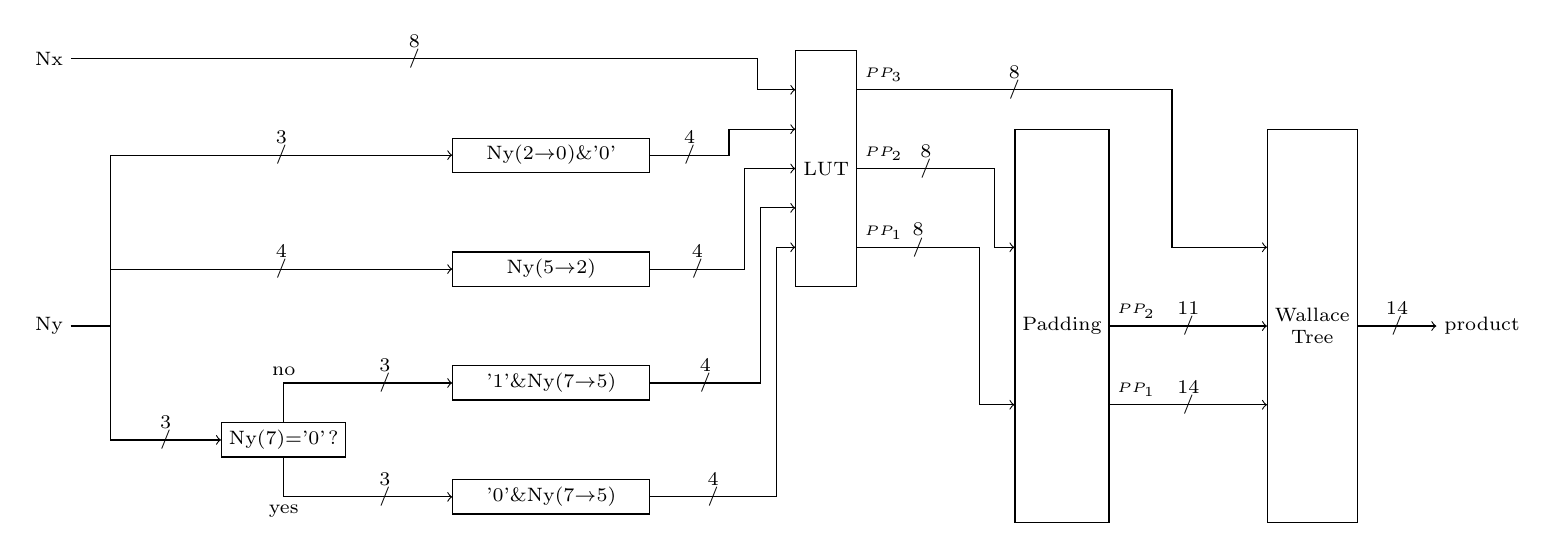
\begin{tikzpicture}[scale=0.5]
\scriptsize

\node [draw,ctrl](c0) {Ny(2$\rightarrow$0)\&'0'};
\node [draw,ctrl, below=of c0](c1) {Ny(5$\rightarrow$2)};
\node [draw,ctrl, below=of c1](c21) {'1'\&Ny(7$\rightarrow$5)};
\node [draw,ctrl, below=of c21](c22) {'0'\&Ny(7$\rightarrow$5)};

\path (c1) -- (c21) node[pos=0.5](middle){};
\node [draw, right=of middle,minimum height=3cm,xshift=2cm,yshift=2cm](lut){LUT};
\node [coordinate,below=0.5cm of lut](lut1){};

\path (c21) -- (c22) node[pos=0.5](middle2){};
\node [draw, left=of middle2,xshift=-1.5cm](c20){Ny(7)='0'?};

\node [draw, right=2cm of lut,minimum height=5cm,yshift=-2cm](pad){Padding};
\node [draw, right=2cm of pad,minimum height=5cm,align=center](wt){Wallace\\Tree};

\draw[->] (c22.east)  -- node(bit12){/} ++(3.2,0) |- ($(lut.west)+(0,-2cm)$);
\draw[->] (c21.east)  -- node(bit13){/} ++(2.8,0) |- ($(lut.west)+(0,-1cm)$);
\draw[->] (c1.east)   -- node(bit14){/} ++(2.4,0) |- ($(lut.west)+(0,0cm)$);
\draw[->] (c0.east)   -- node(bit15){/} ++(2.0,0) |- ($(lut.west)+(0,1cm)$);

\draw[->] (c20.north) |- node[above] {no}  node[pos=0.8](bit4){/}(c21) ;
\draw[->] (c20.south) |- node[below] {yes} node[pos=0.8](bit5){/}(c22);

\node[left=of middle,xshift=-5cm](yin){Ny};
\draw[->] (yin.east) -- ++(1,0) |- node[pos=0.75](bit0){/}(c20);
\draw[->] (yin.east) -- ++(1,0) |- node[pos=0.75](bit1){/}(c1);
\draw[->] (yin.east) -- ++(1,0) |- node[pos=0.75](bit2){/}(c0);

\node[above=of yin, yshift=2cm](xin){Nx};
\draw[->] (xin) -- ++(18cm,0) node[pos=0.5](bit3){/} |- ($(lut.west)+(0,2cm)$);

\draw[->] ($(lut.east)+(0,2cm)$) node[anchor=south west]{\tiny $PP_3$}-- node(bit9){/} ++(8cm,0) |- ($(wt.west)+(0,2cm)$);
\draw[->] ($(lut.east)+(0,0cm)$) node[anchor=south west]{\tiny $PP_2$} -- node(bit10){/} ++(3.5cm,0) |- ($(pad.west)+(0,2cm)$);
\draw[->] ($(lut.east)+(0,-2cm)$)node[anchor=south west]{\tiny $PP_1$} -- node(bit11){/} ++(3.1cm,0) |- ($(pad.west)+(0,-2cm)$);

\draw[->] ($(pad.east)+(0,0cm)$) node[anchor=south west]{\tiny $PP_2$} to node(bit6){/}($(wt.west)+(0,0cm)$);
\draw[->] ($(pad.east)+(0,-2cm)$) node[anchor=south west]{\tiny $PP_1$} to node(bit7){/}($(wt.west)+(0,-2cm)$);

\draw[->] (wt.east) -- node(bit8){/}++(2cm,0) node[anchor=west]{product};

\node at (bit0.north) {3};
\node at (bit1.north) {4};
\node at (bit2.north) {3};
\node at (bit3.north) {8};
\node at (bit4.north) {3};
\node at (bit5.north) {3};
\node at (bit6.north) {11};
\node at (bit7.north) {14};
\node at (bit8.north) {14};
\node at (bit9.north) {8};
\node at (bit10.north) {8};
\node at (bit11.north) {8};
\node at (bit12.north) {4};
\node at (bit13.north) {4};
\node at (bit14.north) {4};
\node at (bit15.north) {4};

\end{tikzpicture}

\end{document}